%!TEX root = ../Thesis.tex
\section*{Anhang}
\addcontentsline{toc}{section}{Anhang}
\fancyhead[R]{Anhang}

\anhangsverzeichnis

\anhang{Gesprächsnotizen}

\subanhang{Gespräch mit Werner Müller}

Gespräch mit Werner Müller am 01.01.2013 zum Thema XXX:
\begin{compactitem}
   \item Über das gute Wetter gesprochen
   \item Die Regenwahrscheinlichkeit liegt immer bei ca. 3\%
   \item Das Unternehmen ist total super
   \item Hier könnte eine wichtige Gesprächsnotiz stehen
\end{compactitem}


\anhang{Abbildungen}
\begin{figure}[h]
    \centering
    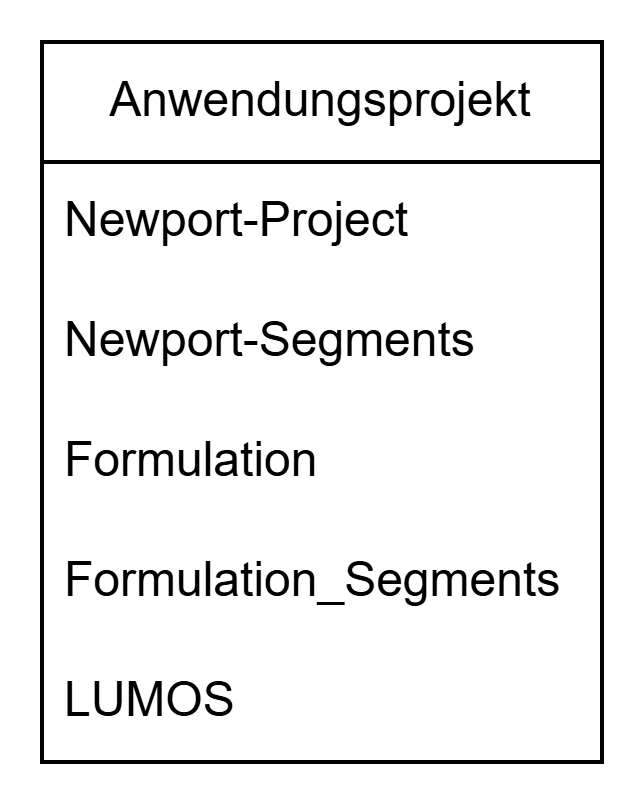
\includegraphics[width=5cm]{./img/projektGrafik.png}
    \caption{projektGrafik}
\end{figure}

\anhang{Listings}
\begin{figure}[H]
    \begin{lstlisting}[caption=JS-Code for the LogIn-Button, breaklines = true, label=list:loginbutton]
        // components/LoginButton.js
        import React from 'react';
        import { useAuth } from '../context/AuthContext';
        import { Button } from '@element/react-components';

        export default function LoginButton() {
            const { login } = useAuth();

            return <Button onClick={login} label="Log In"/>
        }
    \end{lstlisting}
    %\footnoterule{}
    %\footnotesize{Casts have been omitted for the sake of readability}
\end{figure}

\begin{figure}[H]
    \begin{lstlisting}[caption=JS-Code for the LogOut-Button, breaklines = true, label=list:logoutbutton]
        // components/LogoutButton.js
        import React from 'react';
        import { useAuth } from '../context/AuthContext';
        import { Button } from '@element/react-components';

        export default function LogoutButton() {
            const { logout } = useAuth();

            return <Button onClick={logout} label="Log Out"/>
        }
    \end{lstlisting}
    %\footnoterule{}
    %\footnotesize{Casts have been omitted for the sake of readability}
\end{figure}

\begin{figure}[H]
    \begin{lstlisting}[caption=JS-Code for the AuthButton, breaklines = true, label=list:authbutton]
        // components/AuthButton.js
        import React from 'react';
        import { useAuth } from '../context/AuthContext';
        import LoginButton from './LoginButton';
        import LogoutButton from './LogoutButton';

        export default function AuthButton() {
            const { isAuthenticated } = useAuth();

            return isAuthenticated ? <LogoutButton /> : <LoginButton />;
        }
    \end{lstlisting}
    %\footnoterule{}
    %\footnotesize{Casts have been omitted for the sake of readability}
\end{figure}

\begin{figure}[H]
    \begin{lstlisting}[caption=Import und Kontext, breaklines = true, label=list:authcontextimports]
        import React, { createContext, useState, 
        useEffect, useContext } from 'react';
        import { useNavigate, useLocation } from 'react-router-dom';
        import {buildAuthUrl, generateChallenge, generateVerifier, 
        exchangeCodeForTokens} from '../service/authService';
        import authConfig from '../services/authConfig';
        import {generateVerifier, generateChallenge} from '../service/pkce';

        const AuthContext = createContext();
    \end{lstlisting}
\end{figure}

\begin{figure}[H]
    \begin{lstlisting}[caption=Variablen für den Authentifizierungs-Kontext, breaklines = true, label=list:authcontextvariables]
        const [user, setUser] = useState(null);
        const [isAuthenticated, setIsAuthenticated] = useState(false);
        const [tokens, setTokens] = useState(null);
        const navigate = useNavigate();
        const location = useLocation();
    \end{lstlisting}
\end{figure}

\begin{figure}[H]
    \begin{lstlisting}[caption=Login-Methode, breaklines = true, label=list:authcontextlogin]
        async function login() {
            const state = crypto.randomUUID();
            const verifier = generateVerifier();
            const challenge = await generateChallenge(verifier);

            sessionStorage.setItem('oauth_state', state);
            sessionStorage.setItem('pkce_verifier', verifier);
            
            const url = buildAuthUrl({state, code_challenge: challenge});

            window.location.href = url;
        }
\end{lstlisting}
\end{figure}

\begin{figure}[H]
    \begin{lstlisting}[caption=Logout-Methode, breaklines = true, label=list:authcontextlogout]
        function logout() {
            sessionStorage.clear();
            const {logoutEndpoint, clientId, logoutUri} =authConfig;
            window.location.href = `${logoutEndpoint}?client_id=${clientId}&logout_uri=${encodeURIComponent(logoutUri)}`; 
        }
    \end{lstlisting}
\end{figure}

\begin{figure}[H]
    \begin{lstlisting}[caption=Callback-Handling, breaklines = true, label=list:authcontextcallback]
        useEffect(() => {
            if (location.pathname === '/callback' && location.search.includes('code=')) {
                handleCallback();
            }
        }, [location, handleCallback]);
\end{lstlisting}
\end{figure}

\begin{figure}[H]
    \begin{lstlisting}[caption=Callback-Handling, breaklines = true, label=list:authcontextcallback2]
        async function handleCallback() {
            const params = new URLSearchParams(location.search);
            const code = params.get('code');
            const state = params.get('state');
            const saved = sessionStorage.getItem('oauth_state');

            if(!code || !state || state !== saved) {
                return navigate('/', {replace: true});
            }

            try{
                const verifier = sessionStorage.getItem('pkce_verifier');
                const tokenSet = await exchangeCodeForTokens(code, verifier);
                setTokens(tokenSet);

                const [, payload] = tokenSet.id_token.split('.');
                const userInfo = JSON.parse(atob(payload));
                setIsAuthenticated(true);

                sessionStorage.removeItem('pkce_verifier');
                sessionStorage.removeItem('oauth_state');

                navigate('/dashboard', {replace: true});
            } catch (err) {
                console.error('Error during authentication:', err);
                navigate('/', {replace: true});
            }
        }
    \end{lstlisting}
\end{figure}

\begin{figure}[H]
    \begin{lstlisting}[caption=AuthProvider-Komponente, breaklines = true, label=list:authcontextprovider]
        return (
            <AuthContext.Provider 
            value={{ user, isAuthenticated, tokens, login, logout }}>
                {children}
            </AuthContext.Provider>
        );
    }
    export function useAuth() {
        return useContext(AuthContext);
    }
    \end{lstlisting}
\end{figure}

\begin{figure}[H]
    \begin{lstlisting}[caption=AuthConfig, breaklines = true, label=list:authconfig]
        const domain = process.env.REACT_APP_COGNITO_DOMAIN;
        const clientId = process.env.REACT_APP_COGNITO_CLIENT_ID; 
        const redirectUri = process.env.REACT_APP_COGNITO_REDIRECT_URI;
        const logoutUri = process.env.REACT_APP_COGNITO_LOGOUT_URI;
        const apiBaseUrl = process.env.REACT_APP_API_BASE_URL;
        export const authConfig = {
            domain,
            clientId,
            redirectUri,
            logoutUri,
            apiBaseUrl: apiBaseUrl,
            authEndpoint: `https://${domain}/oauth2/authorize`,
            tokenEndpoint: `https://${domain}/oauth2/token`,
            logoutEndpoint: `https://${domain}/logout`,
            responseType: 'code',
            scope: 'openid profile email',
        };
    \end{lstlisting}
\end{figure}

\begin{figure}[H]
    \begin{lstlisting}[caption=Build-Auth Methode, breaklines = true, label=list:buildAuth]
        export function buildAuthUrl({state, code_challenge}) {
            const {
                authorizeEndpoint,
                clientId,
                redirectUri,
                responseType,
                scope
            } = authConfig;
            const params = new URLSearchParams({
                client_id: clientId,
                redirect_uri: redirectUri,
                response_type: responseType,
                scope,
                state,
                code_challenge_method: 'S256',
                code_challenge
            });
            return '${authorizeEndpoint}?{params}';
        }
    \end{lstlisting}
\end{figure}

\begin{figure}[H]
    \begin{lstlisting}[caption=ExchangeCodeForToken Methode, breaklines = true, label=list:exchangecodefortoken]
        export async function exchangeCodeForToken(code, code_verifier){
            const {tokenEndpoint, clientId, redirectUri} = authConfig;

            const params = new URLSearchParams({
                grant_type: 'authorization_code',
                client_id: clientId,
                code,
                redirect_uri: redirectUri,
                code_verifier
            });

            const resp = await fetch(tokenEndpoint, {
                method: 'POST',
                headers: {'Content-Type': 'application/x-www-form-urlencoded' },
                body: params.toString()
            });

            const text = await resp.text();

            if(!resp.ok) throw new Error('Token Exchange failed: $(text)')
            return JSON.parse(text);
        }
    \end{lstlisting}
\end{figure}

\begin{figure}[H]
    \begin{lstlisting}[caption=PKCE-Verifier-Generierung, breaklines = true, label=list:pkceverifier]
        export function generateVerifier() {
            const array = new Uint8Array(32);	
            crypto.getRandomValues(array);
            return Array.from(array, b => ('0'+ b.toString(16)).slice(-2)).join('');
        }
    \end{lstlisting}
\end{figure}

\begin{figure}[H]
    \begin{lstlisting}[caption=PKCE-Challenge-Generierung, breaklines = true, label=list:pkcechallenge]
        export async function generateChallenge(verifier) {
            const encoder = new TextEncoder();
            const data = encoder.encode(verifier);
            const hash = await crypto.subtle.digest('SHA-256', data);
            return btoa(String.fromCharCode(...new Uint8Array(hash)))
                .replace(/\+/g, '-').replace(/\//g, '_').replace(/=+$/, '');
        }
    \end{lstlisting}
\end{figure}

\begin{figure}[H]
    \begin{lstlisting}[caption=PKCE-Challenge-Generierung, breaklines = true, label=list:callApi]
        async function callApi(path, options = {}){
            const url = '${authConfig.apiBaseUrl}${path}';
            const resp = await fetch(url, {
                ...options,
                headers: {
                    'Content-Type': 'application/json',
                    Authorization: 'Bearer ${tokens.access_token}',
                    ...options, headers
                }
            });
            if (!resp.ok) throw 
            new Error('API error ${resp.status}: ${await resp.text()}');
            return resp.json();
        }
    \end{lstlisting}
\end{figure}